\chapter{Implementation of the system}
\section{Technological environment}
The technological environment of programming used in Fantasy project has been the framework \href{https://laravel.com/}{Laravel}, which has an integration with PHP and MySQL.

Thanks to PHP, we have made that the Fantasy project webpage was the most similar to STIMEY's for its following integration in the plataform.

And, with MySQL, we manage the database of the fantasies which students and teachers make, being in control of the property and of the access to the fantasies.

\section{Source code}
Source code of application is in the compressed file that we attached to the task.


\section{Code quality}
To see the quality of the code we used the \href{https://www.sonarqube.org/}{SonarQube} tool.

This tool allows you to check the quality of the code hosted on GitHub online.

\newpage
The results have been the following:
\begin{figure}[h]
	\centering
	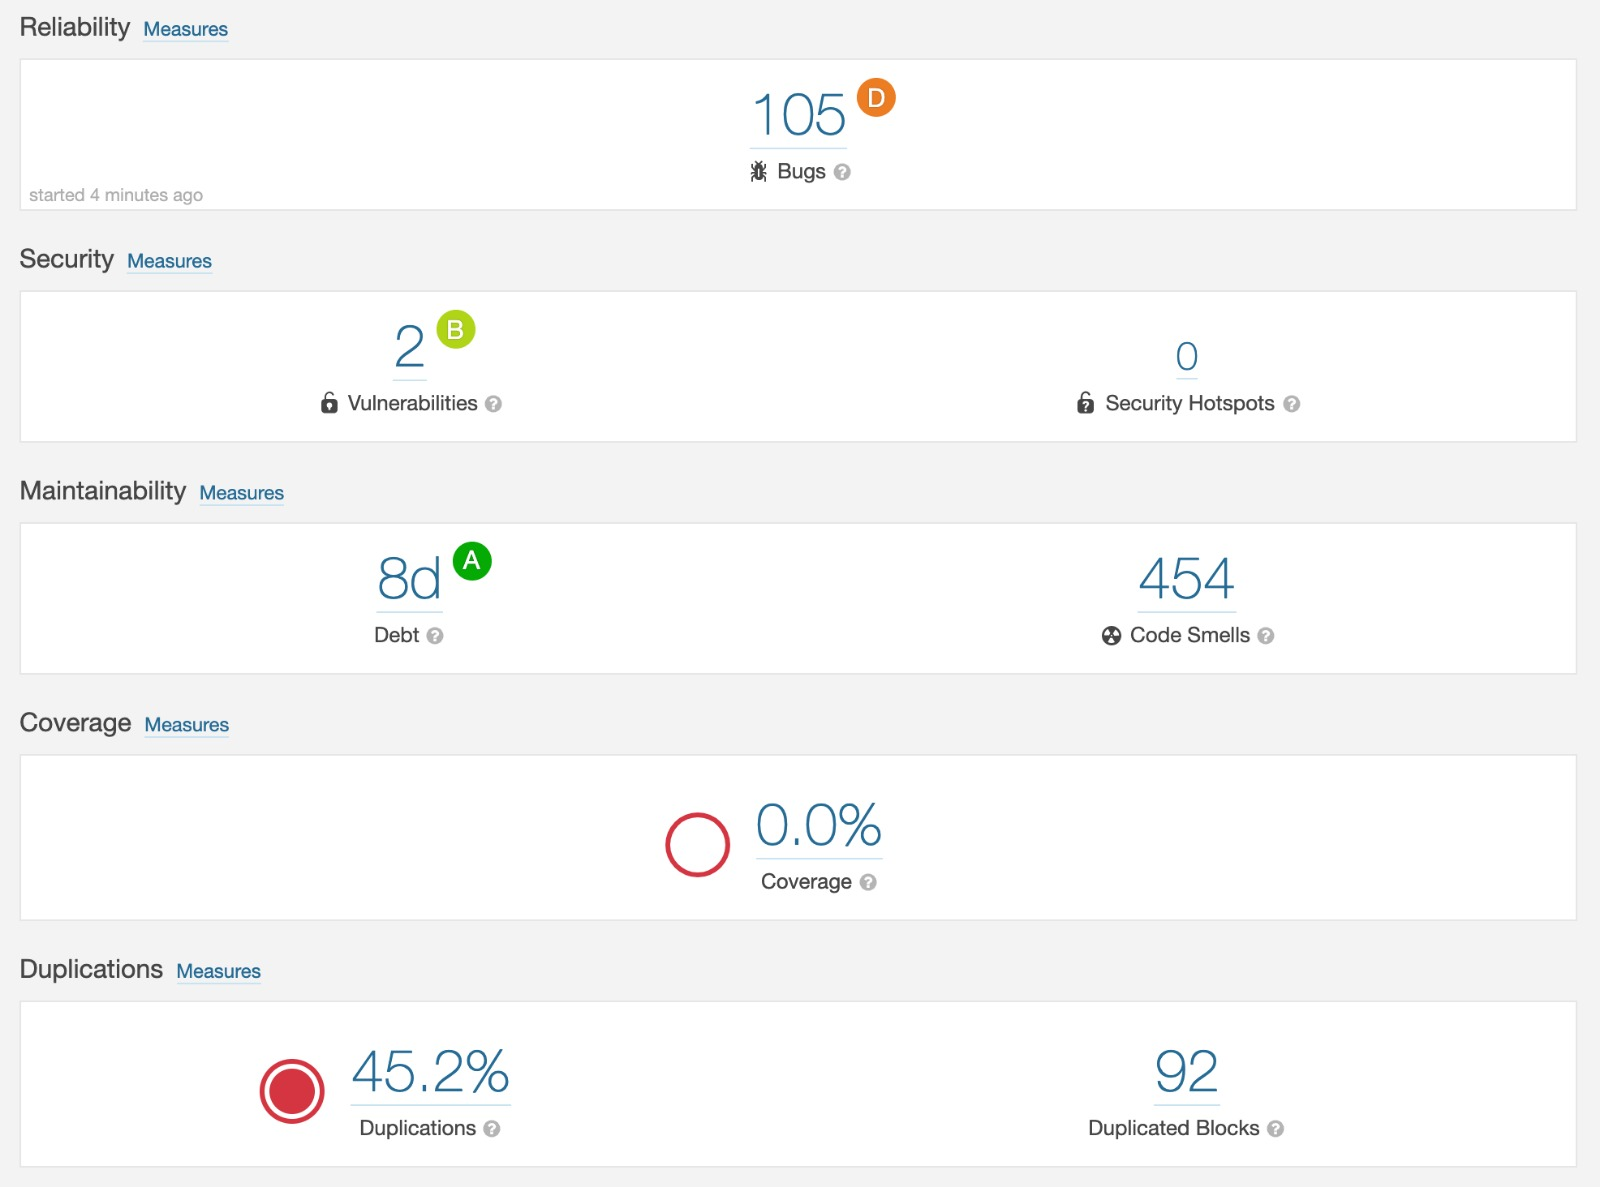
\includegraphics[scale=0.3]{Developing/SQ1.jpeg}
	\caption{SonarQube results.}
	\label{SonarQube results}
\end{figure}
\newpage
\begin{figure}[h]
	\centering
	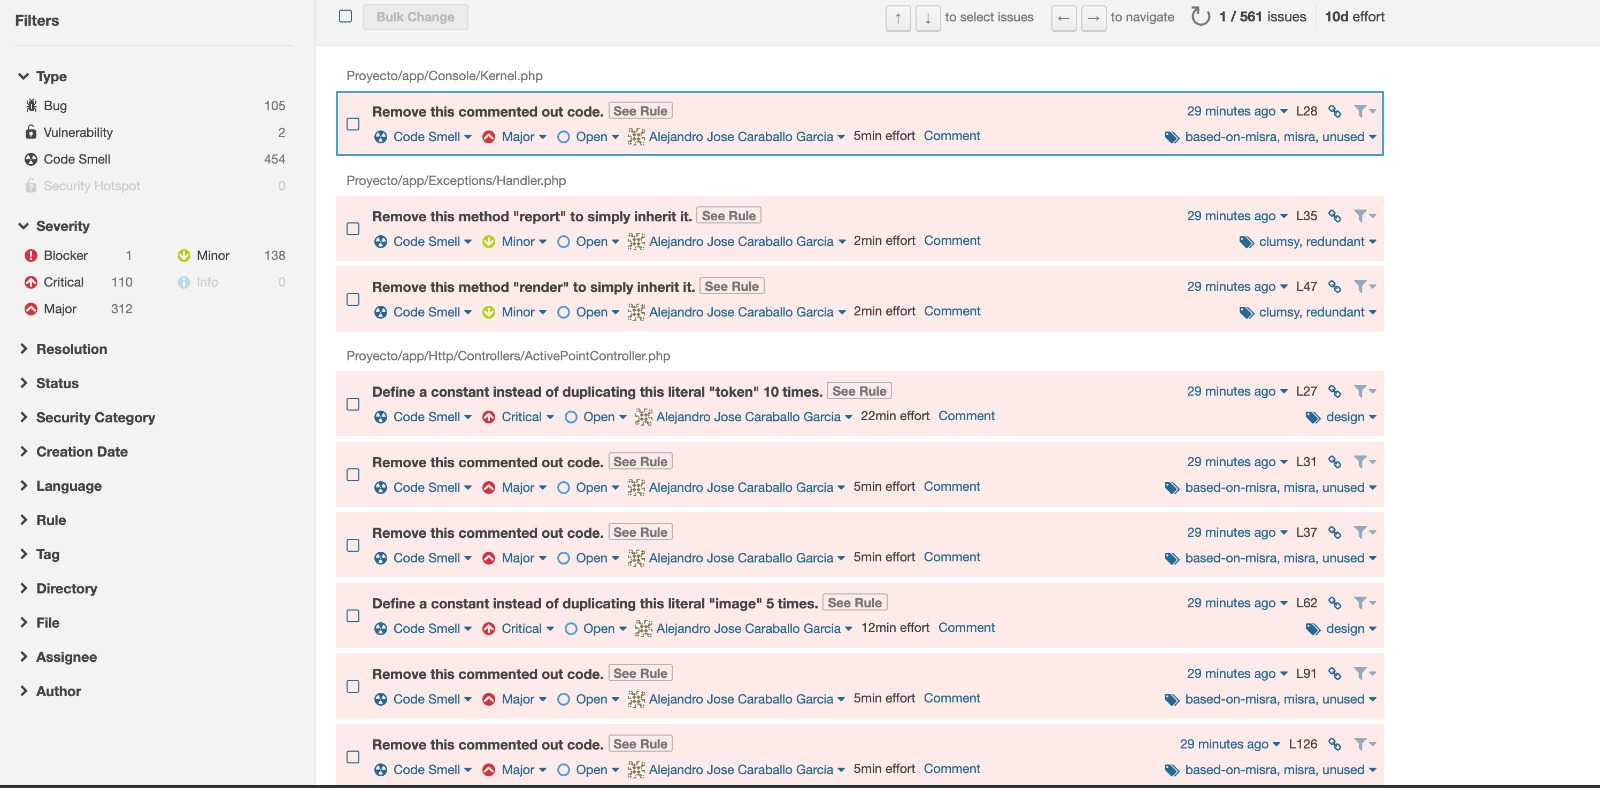
\includegraphics[scale=0.3]{Developing/SQ2.jpeg}
	\caption{SonarQube rules.}
	\label{SonarQube rules}
\end{figure}